%! TEX root = thesis.tex

\chapter{Semiclassical physics}

This chapter is a brief discussion of elastic waves.
In particular, we discuss waves propagating on a filament and shell, both with varying curvatures.
The equations we derive in this chapter would form the basis of our discussions in the next chapter.

\section{WKB analysis}

Consider the differential equation
%
\begin{equation}
  y''(x) + y(x) + \varepsilon \lambda(x) = 0.
\end{equation}
%
Here $\varepsilon$ is a small parameter and suppose we wish to find solutions to this differential equation when $\varepsilon \to 0$.
This is a \emph{regular perturbation} problem because the general characteristic features of this differential equation, namely the fact that it is second order with two independent solutions remains preserved on setting $\varepsilon = 0$.
Hence we can attempt to find a solution of the form
%
\begin{equation}
  y(x) = y_0(x) + \varepsilon y_{1}(x) + \varepsilon^{2} y_{2}(x) + \cdots
\end{equation}
%
Putting this in the original differential equation, we can solve it at different orders of $\varepsilon$ to find
%
\begin{equation}
  \begin{aligned}
    \mathcal{O}(\epsilon^{0}) &: y_{0}''(x) + y_{0}(x) = 0\\
    \mathcal{O}(\epsilon^{1}) &: y_{1}''(x) + y_{0}(x) = 0
  \end{aligned}
\end{equation}
%

The WKB method is a method to find solutions to \emph{singularly perturbed} different equations.

Trouble might occur for instance when

1) the highest order derivative is multiplied by $\varepsilon$.
2) the problem totally changes characteristics when the parameter $\varepsilon$ is equal to zero.
3) the problem is defined on infinite regions.
4) singular points are present.
5) the equation models physical processes with several time- or length scales.

1-5 are called singular perturbation problems.

In many cases we deal with problem containing boundary layers. We can roughly treat these problems by
i) letting  we get a good approximation for the outer region.
ii) rescale the problem to get an inner approximation.
iii) match inner and outer approximations.

Singular perturbation is matched asymptotic expansion.

\section{Diagonalizing multicomponent operators}

Consider a Hermitian linear differential operator $\hat{\mathsf{D}}$ satisfying the wave equation
%
\begin{equation}
  \hat{\mathsf{D}}\Psi = 0,
\end{equation}
%
where $\Psi$ is a multicomponent wave field.
%
We want to find a unitary opeator ${\mathsf{U}}$ such that%
\footnote{It should be emphasized that diagonalizability and unitarity are independent. For instance, let $\mathsf{U}$ be the usual unitary matrix that diagonalizes a matrix $\mathsf{D}$.
  If $\Sigma$ is some nonzero diagonal matrix, not necessarily unitary, then $(\Sigma^{\dagger}\mathsf{U}^{\dagger})\mathsf{D}(\mathsf{U}\Sigma)$ is a diagonal matrix, which follows from the fact that the product of diagonal matrices is diagonal.
  In this sense $\mathsf{U}\Sigma$ can diagonalize $\mathsf{D}$ without being unitary.}
%
\begin{equation}
  \hat{\mathsf{U}}^{\dagger}\hat{\mathsf{D}}\hat{\mathsf{U}} = \hat{\Lambda}\label{eq:diagonalization}
\end{equation}
%
is a diagonal operator.
Clearly, this equivalent to demanding that $\hat{\mathsf{D}}\hat{\mathsf{U}} = \hat{\mathsf{U}}\hat{\Lambda}$.
Let us assume that we can find such an operator and solve the decoupled set of equations given by $\hat{\Lambda}\Phi = 0$.
The solutions to the original equation can then be recovered from $\Phi$ using $\Psi = \hat{\mathsf{U}}\Phi$.
However, Eq.~\eqref{eq:diagonalization} is an equation involving operators and standard linear algebra methods do not (directly) help in finding the unitary operator $\hat{\mathsf{U}}$.

We start by finding the symbol form of the following two equations.
%
\begin{equation}
  \begin{aligned}
    \hat{\mathsf{D}}\hat{\mathsf{U}} &= \hat{\mathsf{U}}\hat{\Lambda}\\
    \hat{\mathsf{U}}^{\dagger}\hat{\mathsf{U}} &= \mathsf{I}_{n}.
  \end{aligned}
\end{equation}
%
Here we assume that the operators $\hat{\mathsf{D}}$, $\hat{\mathsf{U}}$, and $\hat{\Lambda}$ have some problem-relevant ordering parameter $\epsilon$ so that we can expanded the operators (and their symbols) in terms of $\epsilon$.%
\footnote{In their papers, Littlejohn and coworkers~\cite{littlejohn1991,weigert1993} assume that $\hat{\mathsf{D}}$ is \emph{not} ordered in $\epsilon$, i.e., $\hat{\mathsf{D}} = \hat{\mathsf{D}}_{0}$.
  This might seem confusing at first since the parameter $\epsilon$ must appear somewhere in the problem.
  The thing is that very often, $\epsilon$ appears as a factor to a spatial derivative operator, e.g., $-i\epsilon\partial_{x}$, which put together becomes a momentum operator that doesn't have further $\epsilon$ dependence.
  Of course, $\hat{\mathsf{D}}$ could have further nontrivial dependence on $\epsilon$, which is a more general situation, and the one we want to consider here.
}
%
\begin{equation}
  \begin{aligned}
    \hat{\mathsf{D}} &= \hat{\mathsf{D}}_{0} + \epsilon\hat{\mathsf{D}}_{1} + \epsilon^{2}\hat{\mathsf{D}}_{2} + \cdots\\
    \hat{\mathsf{U}} &= \hat{\mathsf{U}}_{0} + \epsilon\hat{\mathsf{U}}_{1} + \epsilon^{2}\hat{\mathsf{U}}_{2} + \cdots\\
    \hat{\Lambda} &= \hat{\mathsf\Lambda}_{0} + \epsilon\hat{\mathsf\Lambda}_{1} + \epsilon^{2}\hat{\mathsf\Lambda}_{2} + \cdots
  \end{aligned}
  \qquad\text{and}\qquad
  \begin{aligned}
    {\mathsf{D}} &= {\mathsf{D}}_{0} + \epsilon{\mathsf{D}}_{1} + \epsilon^{2}{\mathsf{D}}_{2} + \cdots\\
    {\mathsf{U}} &= {\mathsf{U}}_{0} + \epsilon{\mathsf{U}}_{1} + \epsilon^{2}{\mathsf{U}}_{2} + \cdots\\
    {\Lambda} &= {\mathsf\Lambda}_{0} + \epsilon{\mathsf\Lambda}_{1} + \epsilon^{2}{\mathsf\Lambda}_{2} + \cdots
  \end{aligned}
\end{equation}
%
Because the Weyl correspondence preserves Hermiticity, $\mathsf{D}$ is a Hermitian matrix.
We demand that $\Lambda$ remains diagonal at all orders of $\epsilon$.
We then use the Moyal star product to find the symbol form at different orders of $\epsilon$.
At $\mathcal{O}(\epsilon^0)$ we find $\mathsf{D}_{0}\mathsf{U}_{0} = \mathsf{U}_{0}\Lambda_{0}$ and $\mathsf{U}_{0}^{\dagger}\mathsf{U}_{0} = \mathsf{I}_{n}$, which is equivalent to
%
\begin{equation}
  \mathsf{U}_{0}^{\dagger}\mathsf{D}_{0}\mathsf{U}_{0} = \Lambda_{0}.\label{eq:omega0}
\end{equation}
%
Since we demand $\Lambda_{0}$ to be diagonal, this is the usual linear-algebra problem of diagonalizing the matrix $\mathsf{D}_{0}$.
We thus deduce that columns of the lowest order symbol $\mathsf{U}_{0}$ is composed of eigenvectors $\bm{\tau}^{(i)}$ with eigenvalues $\lambda_{0}^{(i)}$ satisfying $\mathsf{D}_{0}\bm{\tau}^{(i)} = \lambda_{0}^{(i)}\bm{\tau}^{(i)}$:
%
\begin{equation}
  \mathsf{U}_{0} =
  \begin{pmatrix}
    \bm{\tau}^{(1)} & \bm{\tau}^{(2)} & \cdots & \bm{\tau}^{(n)}
  \end{pmatrix},
\end{equation}
%
and $\Lambda_{0}$ is the diagonal matrix composed of the eigenvalues $\lambda^{(i)}$.

At $\mathcal{O}(\epsilon^{1})$, demanding $\mathsf{D}\mathsf{U} = \mathsf{U}\Lambda$ gives us
%
\begin{equation}
\mathsf{D}_{1}\mathsf{U}_{0} + \mathsf{D}_{0}\mathsf{U}_{1} + \frac{i}{2}\left\{\mathsf{D}_{0}, \mathsf{U}_{0}\right\} =
  \mathsf{U}_{1}\Lambda_{0} + \mathsf{U}_{0}\Lambda_{1} + \frac{i}{2}\left\{\mathsf{U}_{0}, \Lambda_{0}\right\}.
\end{equation}
%
Multiplying from the left by $\mathsf{U}_{0}^{\dagger}$ and making use of $\mathsf{U}_{0}^{\dagger}\mathsf{D} = \Lambda_{0}\mathsf{U}_{0}^{\dagger}$, we get the $\mathcal{O}(\epsilon)$ correction%
\footnote{For further higher-order corrections to $\Lambda$, see Eq.~(19) of Ref.~\cite{weigert1993}.
Equation~\eqref{eq:omega1} is almost identical to Eqs.~(22)--(24) of Ref.~\cite{venaille2022}, except for the commutator term.
In Ref.~\cite{venaille2022} the commutator term vanishes trivially since $\Lambda_{0}$ is considered to be a scalar.}
%
\begin{equation}
  \Lambda_{1} = \left(\mathsf{U}_{0}^{\dagger}\mathsf{D}_{1}\mathsf{U}_{0} +
  \frac{i}{2}\mathsf{U}_{0}^{\dagger}\left\{\mathsf{D}_{0},\Lambda_{0}\right\} - \frac{i}{2}\mathsf{U}_{0}^{\dagger}\left\{\mathsf{U}_{0},\Lambda_{0}\right\}\right) + \left[\Lambda_{0},\mathsf{U}_{0}^{\dagger}\mathsf{U}_{1}\right].
  \label{eq:omega1}
\end{equation}
%
Above $[~,~]$ denotes the matrix commutator.
We can find $\mathsf{U}_{0}$ and $\Lambda_{0}$ by diagonalizing $\mathsf{D}_{0}$.
The matrix $\mathsf{D}_{1}$ (if it is nonzero) can be found by expanding the symbol matrix $\mathsf{D}$.
But that will not let us find $\Lambda_{1}$ since we still need $\mathsf{U}_{1}$ to evaluate the commutator term $[\Lambda_{0},\mathsf{U}_{0}^{\dagger}\mathsf{U}_{1}]$.
To proceed, we recall that we want $\Lambda$ to be diagonal at all order, which means that $\Lambda_{1}$ must be a diagonal matrix as well.
The $\alpha\beta$th entry of the commutator term evalutes to
%
\begin{equation}
%  \begin{aligned}
    \left[\Lambda_{0},\mathsf{U}_{0}^{\dagger}\mathsf{U}_{1}\right]_{\alpha\beta} = %\Lambda_{0,\alpha\gamma}\left(\mathsf{U}_{0}^{\dagger}\mathsf{U}_{1}\right)_{\gamma\beta} -
  %\left(\mathsf{U}_{0}^{\dagger}\mathsf{U}_{1}\right)_{\alpha\gamma}\Lambda_{0,\gamma\beta}\\
    %&= \lambda_{0}^{(i)}\delta_{\alpha\gamma}\left(\mathsf{U}_{0}^{\dagger}\mathsf{U}_{1}\right)_{\gamma\beta}
  %-\left(\mathsf{U}_{0}^{\dagger}\mathsf{U}_{1}\right)_{\alpha\gamma} \lambda_{0}^{(k)}\delta_{\gamma\beta}\\
    \left[\lambda_{0}^{(i)} - \lambda_{0}^{(j)}\right]\left(\mathsf{U}_{0}^{\dagger}\mathsf{U}_{1}\right)_{\alpha\beta},
%  \end{aligned}
    \label{eq:diagonal}
\end{equation}
%
where we have made use of the fact that $\Lambda_{0}$ is diagonal with $\alpha\beta$th entry $\Lambda_{0,\alpha\beta} = \lambda_{0}^{(i)}\delta_{\alpha\beta}$.
And we see that the diagonal entries (with $\alpha=\beta$) of the commutator vanish.
So the commutator term does not contribute towards the diagonal entries of $\Lambda_{1}$ and we can find the $\mathcal{O}(\epsilon^{1})$ correction $\lambda_{1}$ by carefully evaluating diagonal entries of the remaining terms in the RHS of Eq.~XXX.
Before we do that, we need to discuss the role of the commutator term further.
In fact, without this crucial term, the expansion will break down.

\subsection{Role of the commutator term}

None of our arguments so far guarantees that $\Lambda_{1}$ is diagonal.
In fact, the off-diagonal entries of four matrices in the RHS of Eq.~\eqref{eq:omega1} is generally not equal to zero.
The only way for $\Lambda_{1}$ to be diagonal then is if these off-diagonal entries somehow cancel each other.
We don't have the freedom to choose the off-diagonal entries in the first three terms since they only involve the matrices $\mathsf{U}_{0}$ and $\Lambda_{0}$, both of which are constrained by Eq.~\eqref{eq:omega0}.
However, the commutator term involves the matrix $\mathsf{U}_{1}$, which is something we haven't found yet.
At the same time, $\mathsf{U}_{1}$ isn't a completely arbitrary matrix because on demanding unitarity of $\mathsf{U}$ at $\mathcal{O}(\epsilon)$ we get an additional equation that puts constraints on $\mathsf{U}_{1}$:
%
\begin{equation}
  \mathsf{U}_{0}^{\dagger}\mathsf{U}_{1} + \mathsf{U}_{1}^{\dagger}\mathsf{U}_{0} + \frac{i}{2}\left\{\mathsf{U}_{0}^{\dagger}, \mathsf{U}_{0}\right\}= 0.
  \label{eq:unitarity}
\end{equation}
%
This equation isn't good enough to determine $\mathsf{U}_{1}$ completely, which is good for us since that gives us some freedom in choosing the off-diagonal elements of the commutator term in the way we want.
To simplify the commutator term we first define $\mathsf{X} = \mathsf{U}_{0}^{\dagger}\mathsf{U}_{1}$, and from the previous equation we have
%
\begin{equation}
  \mathsf{X} + \mathsf{X}^{\dagger} = -\frac{i}{2}\left\{\mathsf{U}_{0}^{\dagger}, \mathsf{U}_{0}\right\}.
\end{equation}
%
We see that Hermitian part of $\mathsf{X}$, given by $\mathsf{A} = (\mathsf{X} + \mathsf{X}^{\dagger})/2$, is fixed by the above equation, and $\mathsf{A} = (-i/4)\{\mathsf{U}_{0}^{\dagger},\mathsf{U}_{0}\}$.
This still leaves us with the possibility of picking the anti-Hermitian part of $\mathsf{X}$, which we denote by $i\mathsf{B}$. Here $\mathsf{B}$ is a Hermitian matrix defined by $\mathsf{B} = -i(\mathsf{X} - \mathsf{X}^{\dagger})/2$.\footnote{%
  Writing the anti-Hermitian part of $\mathsf{X}$ this way might look nonstandard and it is more natural to write it as $(\mathsf{X} - \mathsf{X}^{\dagger})/2$.
  This is to ensure that the diagonal entries of matrix $\mathsf{B}$ are real numbers, for the sake of a future argument.
Since the matrices $\mathsf{A}$ and $\mathsf{B}$ are both Hermitian, they have real diagonals.
  These matrices each have $n^{2}$ independent entries composed of $n^{2} - n$ complex off-diagonal entries and $n$ real diagonal entries.
  All $n^{2}$ entries of $\mathsf{A}$ are fixed by $\mathsf{U}_{0}$.
  That leaves us with the freedom to pick the $n^{2}$ remaining entries of $\mathsf{B}$, which is good enough to ensure that $\Omega_{1}$ remains diagonal.
}
After replacing $\mathsf{X} = \mathsf{U}_{0}^{\dagger}\mathsf{U}_{1}$ in the commutator term with $\mathsf{A} + i\mathsf{B}$ and using Eqs.~\eqref{eq:omega1} and \eqref{eq:diagonal}, we can find the off-diagonal entries of $\mathsf{B}$ that will ensure that $\Lambda_{1}$ remains a diagonal matrix:
%
\begin{equation}
  \mathsf{B}_{\alpha\beta} = i\frac{\mathsf{Q}_{\alpha\beta}}{\lambda_{0}^{(\alpha)} - \lambda_{0}^{(\beta)}},
  \quad \text{with }\alpha \neq \beta,
\end{equation}
%
where
%
\begin{equation}
  \mathsf{Q} = \mathsf{U}_{0}^{\dagger}\mathsf{H}_{1}\mathsf{U}_{0} + \frac{i}{2}\mathsf{U}_{0}^{\dagger}\left\{\mathsf{D}_{0},\mathsf{U}_{0}\right\} - \frac{i}{2}\mathsf{U}_{0}^{\dagger}\left\{\mathsf{U}_{0},\Lambda_{0}\right\}
  -\frac{i}{4}\Lambda\left\{\mathsf{U}_{0}^{\dagger}, \mathsf{U}_{0}\right\} +
  \frac{i}{4}\left\{\mathsf{U}_{0}^{\dagger}, \mathsf{U}_{0}\right\}\Lambda.
\end{equation}
%
Although we have found an expression that gives the off-diagonal elements of $\mathsf{B}$, nothing in our arguments so far guaratees the Hermiticity of $\mathsf{B}$ and we have to explicitly check this.%
\footnote{Littlejohn and coworkers~\cite{littlejohn1991,weigert1993} seem to not have stressed this subtle point in their papers and they do not prove the Hermiticity of $\mathsf{B}$ explicitly.
  At first glance, we might think that $\mathsf{B}$ would Hermitian by construction because we \emph{took} $\mathsf{\mathsf{A}}$ and $i\mathsf{B}$ to be the Hermitian and anti-Hermitian parts of $\mathsf{X}$.
  This is not true however, as we obtained $\mathsf{A}$ from requiring unitarity of $\mathsf{U}$ at $\mathcal{O}(\epsilon)$ and we are now attempting to find $\mathsf{B}$ from Eq.~XXX, which is an independent equation that guarantees the diagonalizability of $\mathsf{D}$ at $\mathcal{O}(\epsilon)$.
  However, there is no obvious reason why unitarity at $\mathcal{O}(\epsilon)$ should be compatible with diagonalizability at $\mathcal{O}(\epsilon)$.
  Indeed, we still need an additional requirement, i.e., the Hermiticity of $\mathsf{D}_{1}$, for $\mathsf{B}$ to be Hermitian.
}
From Eq.~XXX, we see that the matrix $\mathsf{Q}$ should be Hermitian if $\mathsf{B}$ is to be Hermitian.
For two general matrices $\mathsf{F}$ and $\mathsf{G}$ we have $\{\mathsf{F},\mathsf{G}\}^{\dagger} = -\{\mathsf{G}^{\dagger},\mathsf{H}^{\dagger}\}$
Along with the assumption that $\mathsf{D}_{1}$ is Hermitian, we then find,
%
\begin{equation}
  \mathsf{Q}^{\dagger} =  \mathsf{U}_{0}^{\dagger}\mathsf{D}_{1}\mathsf{U}_{0} + \frac{i}{2}\left\{\mathsf{U}_{0}^{\dagger},   \mathsf{D}_{0}\right\}\mathsf{U}_{0} - \frac{i}{2}\left\{\Lambda_{0}, \mathsf{U}_{0}^{\dagger}\right\}\mathsf{U}_{0}
  - \frac{i}{4}\left\{\mathsf{U}_{0}^{\dagger}, \mathsf{U}_{0}\right\}\Lambda
  + \frac{i}{4}\Lambda\left\{\mathsf{U}_{0}^{\dagger}, \mathsf{U}_{0}\right\},
\end{equation}
%
which can be further simplified to show that $\mathsf{Q}^{\dagger} = \mathsf{Q}$,%
\footnote{The simplification proceeds (by explicitly computing matrix entries) by first showing that
  $\{\mathsf{U}_{0}^{\dagger}, \mathsf{D}_{0}\}\mathsf{U}_{0} = \{\mathsf{U}_{0}^{\dagger}, \mathsf{U}_{0}\}\Lambda - \mathsf{U}_{0}^{\dagger}\{\mathsf{U}_{0}, \Lambda\} - \{ ^{1}\mathsf{U}_{0}^{\dagger}, ^{3}\mathsf{U}_{0}\}^{2}\mathsf{D}_{0}$,
  and
  $\{\Lambda_{0}, \mathsf{U}_{0}^{\dagger}\} = \Lambda_{0}\{\mathsf{U}_{0}^{\dagger},\mathsf{U}_{0}\} - \mathsf{U}_{0}^{\dagger}\{\mathsf{D}_{0},\mathsf{U}_{0}\} - \{^{1}\mathsf{U}_{0}^{\dagger},^{3}\mathsf{U}_{0}\}^{2}\mathsf{D}_{0}$.
  Here the superscripts 1, 2, and 3 appearing before the matrices denote the order in which they are to be multiplied.
  Upon using these results in the RHS of Eq.~XXX, we see that $\mathsf{Q}=\mathsf{Q}^{\dagger}$.
}
from which the Hermiticity of $\mathsf{B}$ follows.

Clearly, our scheme would break down if the symbol matrix $\mathsf{D}$ has an $\mathcal{O}(\epsilon^{0})$ degeneracy, i.e., if $\mathsf{D}_{0}$ is degenerate with $\lambda_{0}^{(\alpha)} = \lambda_{0}^{(\beta)}$ for some $\alpha \neq \beta$.
Clearly, we cannot determine the diagonal entries $\mathsf{B}_{\alpha\alpha}$ from our results so far.
However, we can always take them to be zero, since they do not affect the unitarity of $\mathsf{U}$ to $\mathcal{O}(\epsilon)$.
The symbol matrix $\mathsf{U}$ to $\mathcal{O}(\epsilon)$ is
%
\begin{equation}
  \mathsf{U} = \mathsf{U}_{0} + \epsilon \mathsf{U}_{1} + \mathcal{O}(\epsilon^{2}) = \mathsf{U}_{0}\left[\mathsf{I}_{n} + \epsilon\left(\mathsf{A} + i\mathsf{B}' + i\mathsf{B}'' \right)\right] + \mathcal{O}(\epsilon^{2}),
\end{equation}
%
where we made use of $\mathsf{U}_{1} = \mathsf{U}_{0}(\mathsf{A} + i\mathsf{B})$ and wrote $\mathsf{B}$ as the sum of its diagonal part $\mathsf{B}'$ and off-diagonal part $\mathsf{B}''$.%
\footnote{Since $\mathsf{B}$ is Hermitian, its diagonal part $\mathsf{B}'$ is a real matrix.}
Now, note that we have complete freedom in choosing phase factors for the columns of $\mathsf{U}_{0}$, namely the eigenvectors of $\mathsf{D}_{0}$.
Rephasing the $\alpha$th column by $e^{-i\epsilon\mathsf{B}'_{\alpha\alpha}}$ turns
%
\begin{equation}
    \mathsf{U}_{0} \to
      \begin{pmatrix}
        e^{-i\epsilon\mathsf{B}'_{11}}\bm{\tau}^{(1)} &
        e^{-i\epsilon\mathsf{B}'_{22}}\bm{\tau}^{(2)} &
        \cdots &
        e^{-i\epsilon\mathsf{B}'_{nn}}\bm{\tau}^{(n)} &
      \end{pmatrix}
      = \mathsf{U}_{0}(\mathsf{I}_{n} - i\epsilon\mathsf{B}') + \mathcal{O}(\epsilon^{2})
\end{equation}
%
Under the gauge transformation, the matrices $\mathsf{A} \to \mathsf{A} + \mathcal{O}(\epsilon)$ and $\mathsf{B}'' \to \mathsf{B}'' + \mathcal{O}(\epsilon)$.
Thus, the RHS of Eq.~XXX becomes
%
\begin{equation}
  \left[\mathsf{U}_{0}(\mathsf{I}_{n} - i\epsilon\mathsf{B}') + \mathcal{O}(\epsilon^{2})\right]\left[\mathsf{I}_{n} + \epsilon\left(\mathsf{A} + i\mathsf{B}' + i\mathsf{B}'' + \mathcal{O}(\epsilon)\right)\right]
  =
  \mathsf{U}_{0}\left[\mathsf{I}_{n} + \epsilon\left(\mathsf{A} + i\mathsf{B}'' \right)\right] + \mathcal{O}(\epsilon^{2}).
\end{equation}
%
In other words, we can obsorb any nonzero diagonal entries of $\mathsf{B}$ by a suitable rephasing of the columns of $\mathsf{U}_{0}$.
Thus, without loss of generality we take the diagonal part $\mathsf{B}'$ to be zero.

\begin{example}[A simple ``coupled'' differential operator]
Consider an operator $\hat{\mathsf{D}}$ (with symbol $\mathsf{D}$) defined by
%
\begin{equation}
  \hat{\mathsf{D}} =
  \begin{pmatrix}
    \hat{p} & -\lambda\\
    -\lambda & \hat{p}
  \end{pmatrix}
  \qquad\text{and}\qquad
  \mathsf{D} =
  \begin{pmatrix}
    p & -\lambda\\
    -\lambda & p
  \end{pmatrix}.
\end{equation}
%
The wave equation $\hat{\mathsf{D}}\Psi = 0$ defined by this operator can be trivially shown to be equivalent to the uncoupled ODEs $\partial_{x}^{2}\Psi_{\alpha} + \lambda^{2}\Psi_{\alpha} = 0$ in components $\Psi_{\alpha}$ of $\Psi$.
Solving this ODE, we find $\Psi_{1} = A_{+}e^{i \lambda x} + A_{-}e^{-i\lambda x}$ and $\Psi_{2} = A_{+}e^{i \lambda x} - A_{-}e^{-i\lambda x}$.
%
By diagonalizing the symbol matrix $\mathsf{D}$, we find $\mathsf{U}$ and $\Lambda$, which can be transformed back to find the diagonalized operator $\hat{\Lambda}$:
%
\begin{equation}
  \mathsf{U} = \frac{1}{\sqrt{2}}
  \begin{pmatrix}
    1 & 1\\
    1 & -1
  \end{pmatrix},\enspace
  \Lambda =
  \begin{pmatrix}
    p - \lambda & 0\\
    0 & p + \lambda
  \end{pmatrix},\enspace
  \text{and}\enspace
  \hat{\Lambda} =
  \begin{pmatrix}
    \hat{p} - \lambda & 0\\
    0 & \hat{p} + \lambda
  \end{pmatrix}.
\end{equation}
%
The uncoupled system given by $\hat{\Lambda}\Phi = 0 $ has solutions $\Phi_{1} = B_{+}e^{i\lambda x}$ and $\Phi_{2} = B_{-}e^{-i\lambda x}$.
The solution to the original system can be recovered by $\Psi = \hat{\mathsf{U}}\Phi$, which gives us\footnote{The operator $\hat{\mathsf{U}}$ is equal to its symbol $\mathsf{U}$ since its matrix entries are constants.}
%
\begin{equation}
  \Psi = \frac{1}{\sqrt{2}}
  \begin{pmatrix}
    1 & 1\\
    1 & -1
  \end{pmatrix}
  \begin{pmatrix}
    B_{+}e^{i\lambda x}\\
    B_{-}e^{-i\lambda x}
  \end{pmatrix}
  =
  \begin{pmatrix}
    A_{+}e^{i\lambda x} + A_{-}e^{-i\lambda x}\\
    A_{+}e^{i\lambda x} - A_{-}e^{-i\lambda x}
  \end{pmatrix},
\end{equation}
%
where we have set $A_{\pm} = B_{\pm}/\sqrt{2}$, and have found the expected solution.
\end{example}

\section{Wave dynamics and supersymmetry}

Consider a Hermitian linear differential operator $\hat{\mathsf{D}}$ satisfying the wave equation
%
\begin{equation}
  -\partial_{t}^{2}\Psi = \hat{\mathsf{D}}\Psi.
\end{equation}
%
Although this equation is second-order in time, we can cast it as two sets of coupled differential equations that are first order in time by defining $\dot{\Psi} = \partial_{t}\Psi$, so that
%
\begin{equation}
  \partial_{t}
  \begin{pmatrix}
    \Psi \\
    \dot{\Psi}
  \end{pmatrix}
  =
  \begin{pmatrix}
    0 & 1\\
    -\hat{\mathsf{D}} & 0
  \end{pmatrix}
  \begin{pmatrix}
    \Psi \\
    \dot{\Psi}
  \end{pmatrix}.
\end{equation}
%
There's nothing special about recasting the equations this way, and indeed every wave equation (even nonlinear ones) can be rewritten this way.
There are also problems -- the wave operator that we are left with is no longer Hermitian (or even anti-Hermitian).
However, if we can write $\hat{\mathsf{D}} = \hat{\mathsf{Q}}\trans\hat{\mathsf{Q}}$, instead of considering the above equation, we could instead consider the equation for a transformed field
\begin{equation}
  \Phi = \hat{\mathsf{T}}
  \begin{pmatrix}
    \Psi\\
    \dot{\Psi}
  \end{pmatrix}
\end{equation}
%
where
%
\begin{equation}
  \hat{\mathsf{T}} =
  \begin{pmatrix}
    \hat{\mathsf{Q}} & 0\\
    0 & i
  \end{pmatrix}.
\end{equation}
%
Differentiating Eq.~XXX with respect to time and making use of Eq.~XXX, we find the Schr\"{o}dinger-like equation\footnote{Note that only spatial derivatives appear in $\hat{\mathsf{T}}$, so that $\partial_{t}\hat{\mathsf{T}} = \hat{\mathsf{T}}\partial_{t}$.}
%
\begin{equation}
  i\partial_{t}\Phi =
  \begin{pmatrix}
    0 & \hat{\mathsf{Q}}\\
    \hat{\mathsf{Q}}\trans & 0
  \end{pmatrix}
  \Phi.
\end{equation}

\section{Multicomponent wave equations}

\subsection{A multicomponent eigenvalue problem}

In this section we will apply the results that we derived previously to a multicomponent problem whose solution is known exactly.
Consider the following multicomponent eigenvalue problem%
\footnote{These equations are slightly modified versions of the channel equations considered by~\citet{yabana1986}.}
%
\begin{equation}
  \begin{bmatrix}
    \left(\hat{a}^{\dagger}\hat{a} + \frac{1}{2}\right)\epsilon + \Delta & \mu\hat{a}^{\dagger}\\
    \mu\hat{a} & \left(a^{\dagger}\hat{a} + \frac{1}{2}\right)\epsilon - \Delta
  \end{bmatrix}
  \begin{bmatrix}
    \psi_{+}\\
    \psi_{-}
  \end{bmatrix}
  =
  E
  \begin{bmatrix}
    \psi_{+}\\
    \psi_{-}
  \end{bmatrix}.
\end{equation}
%
Above, $\Delta$ is a positive constant and the operators
%
\begin{equation}
\hat{a}^{\dagger} = \frac{x - i\hat{k}}{\sqrt{2\epsilon}}
  \quad\text{and}\quad
\hat{a} = \frac{x + i\hat{k}}{\sqrt{2\epsilon}},
\end{equation}
%
are the usual raising and lowering operators from quantum mechanics.%
\footnote{Here the parameter $\epsilon$ plays the role of the Planck's constant and we have set the mass and oscillator frequency to unity.}
Without the off diagonal terms, these equations reduce to two uncoupled simple harmonic oscillators, in which case the energies would be given by $E_{n}^{\pm} = (n + \frac{1}{2})\epsilon \pm \Delta$ for $n \in \mathbb{N}_{0}$.
To solve the eigenvalue problem in the presence of off-diagonal term, we expand the solution in terms of the eigenstates of the simple harmonic oscillator
%
\begin{equation}
  \psi_{+} = \sum_{n= 0}^{\infty} a_{n}\phi_{n}
  \quad\text{and}\quad
  \psi_{-} = \sum_{n = 0}^{\infty} b_{n}\phi_{n}.
\end{equation}
%
Putting the above equation in Eq.~XXX, we arrive at
%
\begin{equation}
   \begin{aligned}
     \sum_{n = 0}^{\infty} \left\{\left[\left(n +  \tfrac{3}{2}\right)\epsilon + \Delta - E\right]a_{n + 1} + \sqrt{n + 1}b_{n}\right\}\phi_{n+1}  + a_{0}\left(\tfrac{1}{2}\epsilon + \Delta - E\right)\phi_{0}&= 0\\
     \sum_{n = 0}^{\infty} \left\{\sqrt{n + 1}a_{n+1} + \left[\left(n +  \tfrac{1}{2}\right)\epsilon - \Delta - E\right]b_{n}\right\}\phi_{n} &= 0.
   \end{aligned}
\end{equation}
%
Since the $\phi_{n}$ are independent functions, their coefficients in the above equations should independently vanish, which leads us to the quantization condition.
Clearly, the lowest energy is $E = \tfrac{1}{2}\epsilon + \Delta$ and the associated eigenstate is $\psi = (0, \phi_{0})$.
%
\begin{equation}
  \begin{bmatrix}
    \left(n + \tfrac{1}{2}\right)\epsilon - \Delta - E & \sqrt{n + 1}\\
    \sqrt{n + 1} & \left(n + \tfrac{3}{2}\right) + \Delta - E
  \end{bmatrix}
  \begin{bmatrix}
    a_{n}\\
    b_{n + 1}
  \end{bmatrix}
  = 0.
\end{equation}
%

\section{Filament equations}

%
\begin{equation}
  \mathscr{E}[\zeta, u] = \mathscr{K} - \mathscr{U} = \int \dd{t}\,\dd{x}\,\frac{1}{2}\left\{\rho\left(\dot{u}^{2} + \dot{\zeta}^{2}\right) - A\left[u' - m(x)\zeta\right]^{2} - B\left(\zeta''\right)^{2}\right\}
\end{equation}
%
\begin{figure}
  \begin{center}
    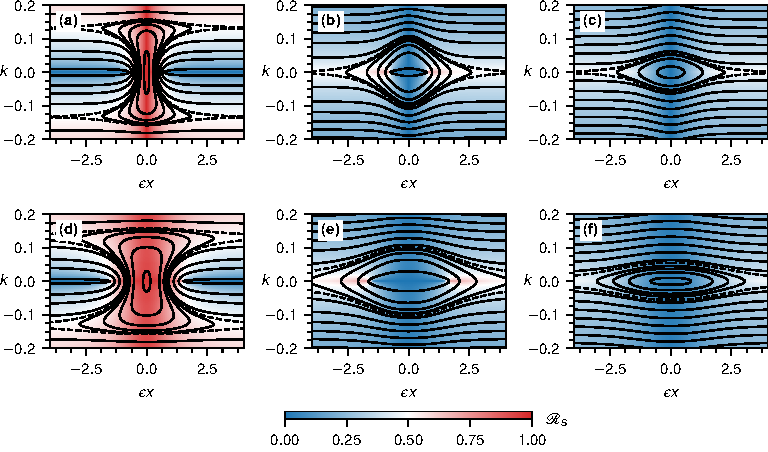
\includegraphics{shell_rays.pdf}
  \end{center}
\end{figure}

